\subsection{Definición y propiedades generales}

\begin{definition}[Dominio euclídeo]
	Un dominio de integridad $A$ es un dominio euclídeo si existe una función euclídea $\phi:A \setminus \{0\} \to \mathbb{N}$ tal que:
	
	\begin{enumerate}
	\item $\forall a,b \in A \setminus \{0\}. \phi(ab) \ge \phi(b)$
	\item $\forall a,b \in A,b \neq 0. \exists q,r \in A. a = bq + r$ con $r = 0$ o $\phi(r) < \phi(b)$.
	\end{enumerate}
	
	En la propiedad anterior, $q$ se llama cociente y $r$ se llama resto. La segunda condición puede restringirse a la comprobación de la siguiente propiedad: 
	
	$\forall a,b \neq 0. \phi(a) \ge \phi(b). \exists q,r \in A. a = bq + r$ con $r = 0$ o $\phi(r) < \phi(b)$
	
	con lo que nos quitamos los casos $a = b0 + a \land 0 = b0 + 0$. Equivalentemente:
	
	$\forall a,b \neq 0. \phi(a) \ge \phi(b). \exists q \in A. a = bq \lor \phi(a-bq) < \phi(b)$
\end{definition}

\begin{example}[Cualquier cuerpo es un dominio euclídeo]

En efecto, si $K$ es un cuerpo, la función euclídea es $\phi: K \setminus \{0\} \to \mathbb{N}$ tal que $\phi(k) = 1$. 

Se verifica que $\forall a,b \in A \setminus \{0\}.\phi(ab) \ge \phi(b)$. Además, $\forall a,b \in A, b \neq 0. q = a b^{-1} \land r = 0 \implies a = qb + r$.
\end{example}

\begin{proposition}[Caracterización de la divisibilidad en dominios euclídeos]
	Dado $A$ un dominio euclídeo. 
	
	$b | a \iff \exists q \in A. a = bq$ esto es, todo resto euclídeo de la división de $a$ entre $b$ es cero. 
\end{proposition}
\begin{proof}
	$\Rightarrow)$ Como $b|a \implies \exists c \in A. a = bc$ y como $A$ es un dominio euclídeo $\exists q,r. a = bq + r$ con $r = 0 \lor \phi(r) < \phi(b)$. Si $r = 0$ hemos acabado. En otro caso, suponemos $r \neq 0$ y por tanto debe ser $\phi(r) < \phi(b)$. 
	
	Claramente, $bc = bq + r $ y por tanto $r = b(c-q)$. Tomando $\phi$, tenemos que $\phi(r) = \phi(b(c-q)) \ge \phi(b) > \phi(r)$ por hipótesis y llegamos a una contradicción. Por tanto debe ser, $r = 0$. 
	
	$\Leftarrow)$ Trivial. 
\end{proof}

\subsection{Dominio euclídeo de los enteros}

\begin{theorem}[Teorema de Euclides]
$\mathbb{Z}$ es un dominio euclídeo con:
	
\begin{enumerate}
\item Función euclídea el valor absoluto. 
\item Unicidad del cociente y unicidad  del resto sobre $\mathbb{N}$. 
\end{enumerate} 
	
hay que notar que la unicidad de este resultado es impuesta en el sentido de que los restos son únicos si sólo se consideran válidos sobre $\mathbb{N}$ y no sobre $\mathbb{Z}$ como permite la definición de dominio euclídeo. 
\end{theorem}
\begin{proof}
	1. Claramente, $\forall a,b \in A. \phi(ab) = |ab| \ge |b| = \phi(b)$.\\
	2. Sea $b > 0$ y consideremos el conjunto de posibles restos positivos que pueden quedar al dividir por $b$, esto es, $R = \{a-bx:x\in \mathbb{Z}\} \cap \mathbb{N}$. Vamos a elegir como $r$ el mínimo de este conjunto. 
	
	Primero vemos que $R \neq \emptyset$. Para ello basta elegir $x = - |a|$ de modo que el correspondiente elemento del conjunto es $a + b|a|$. Distinguimos dos casos:
	
	\begin{itemize}
		\item Si $a > 0 \implies a+b|a| = a+ba = a(1+b) \ge 0$.
		\item Si $a < 0 \implies a+b|a| = a-ba = a(1-b) \ge 0$. 
	\end{itemize}
	
	Por tanto $a+b|a| \in R$ y como $\mathbb{N}$ es bien ordenado tenemos que $R$ tiene un mínimo. Definimos $r = min R$. Como $r \in R$ claramente $r \ge 0$ y $\exists q \in \mathbb{Z}. r = a-bq \implies a = bq + r$. Terminamos la demostración para este caso, garantizando que $r < |b| = b$. Pero esto es fácil ya que si $r \ge b$ entonces $r-b = a-b(q+1) \implies r-b \in R$ y como $r-b < r$ tenemos contradicción con la definición de $r$. Por tanto se verifica que $r < |b|$. 
	
	Si $b < 0$ entonces se transforma al caso $b > 0$. Se resuelve el problema para $a$ y $-b$ obteniendo una expresión $a = (-b)q+r$ con $0 \leq r < |-b|$ de donde $a = b(-q) + r$ y claramente $0 \leq r < |b|$ ya que $|-b| = |b|$. 
	
	Finalmente, veamos que el cociente y el resto son únicos.  Para ello escribamos $$a = bq + r = bq'+r' \text{ con } 0 \le r < |b| \land 0 \le r' < |b| \implies b(q'-q) = r' - r \implies |b| \le |q' - q||b| = |r'-r|$$ donde la última desigualdad se cumple por el carácter multiplicativo del valor absoluto. Obsérvese que estamos asumiendo implícitamente que $q \neq q' \land r \neq r'$ para poder tomar valores absolutos en la definición de dominio euclídeo. Si los cocientes son iguales es fácil deducir que los restos son iguales y viceversa teniendo en cuenta que $\mathbb{Z}$ es un dominio de integridad. 
	
	Sin embargo, por las condiciones que cumplen $r$ y $r'$ tendríamos que: $$0 \le r < |b| \land -|b| < -r' \le 0 \implies -|b| < r' - r < |b| \implies |r'-r| < |b|$$ Ambas desigualdades son contradictorias.
\end{proof}

El conjunto $R = \{a-bx:x \in \mathbb{Z}\} \cap \mathbb{N}$ no es directamente computable. Pero si $a,b > 0$ bastaría con comprobar una lista de números naturales comenzando en cero para hallar el menor elemento del conjunto (que existe y es único por el teorema anterior). Entonces conviene definir el siguiente procedimiento algorítmico para calcular los restantes casos:

\begin{theorem}[Algoritmo de división]
	\begin{itemize}
		\item Si $a,b > 0$ se procede del modo habitual. 
		\item En otro caso los resultados se obtienen al dividir los correspondientes positivos:
		\begin{itemize}
			\item Si $r = 0 \land a = bq$
			
			\begin{itemize}
				\item Si $a,b < 0$ entonces $-a = (-b)q$
				\item Si $a < 0$ entonces $-a = b(-q)$
				\item Si $b < 0$ entonces $a = (-b)(-q)$.
			\end{itemize}
			\item Si $r > 0 \land r < b, a = bq+r$
			
			\begin{itemize}
				\item Si $a,b < 0$ entonces $-a = (-b)(q+1)+(b-r)$.
				\item Si $a < 0$ entonces $-a = b(-q-1)+(b-r)$.
				\item Si $b < 0$ entonces $a = (-b)(-q)+r$. 
			\end{itemize}
		\end{itemize}
	\end{itemize}
\end{theorem}

\subsection{Dominio euclídeo de los polinomios con coeficientes en un cuerpo.}

\subsubsection{Demostración basada en un algoritmo de división sobre dominios de integridad}

\begin{lemma}[División de polinomios en dominios de integridad]
	Dado $A$ un dominio de integridad. 
	
	$\forall f,g \in A[X]$ donde el coeficiente líder de $g$ es unidad del anillo, $\exists!q,r \in A[X]. f = gq + r$ con $r = 0$ o $gr(r) < gr(g)$. 
\end{lemma}
\begin{proof}
	Sean $f = \sum_{i=0}^{n} a_ix^i$ con $a_n \neq 0$ y $g = \sum_{i = 0}^{m} b_jx^j$ con $b_m \in U(A)$. Ahora, 
	
	\begin{itemize}
		\item Si $n < m$ entonces $f(x) = g(x)0 + f(x)$. 
		\item Si $n \ge m$ entonces hacemos inducción fuerte sobre $n$. 
		
		\begin{itemize}
			\item Si $n = 0$ entonces $f = a_0 \land g = b_0 \in U(A)$ y por tanto podemos escribir $f = a_0 = b_0(b_0^{-1}a_0) + 0$. 
			\item Si $n > 0$ podemos considerar $f_1 = f - a_nb_m^{-1}x^{n-m}g$ esto es el polinomio que resulta al restar apropiadamente el divisor $g$ poniendole como coeficiente el coeficiente de grado $n$ del polinomio $f$. Claramente, $gr(f_1(x)) < gr(f(x))$ y por hipótesis de inducción $\exists!q_1,r_1 \in A[X]. f_1 = gq_1+r_1$ con $r_1 = 0$ o $gr(r_1) < gr(g)$. 
			
			Usando la anterior descomposición hallamos la descomposición para $f$ como: $$f = f_1(x) = a_1b_m^{-1}x^{n-m}g = gq_1 + r_1 + a_nb_m^{-1}x^{n-m}g = g(q_1+a_nb_m^{-1}x^{n-m}+r_1$$ Y llamamos $q = q_1+a_nb_m^{-1}x^{n-m} \land r = r_1$ y por tanto $r = 0 \lor gr(r) < gr(g)$.  
		\end{itemize}
	\end{itemize}
	
	Finalmente, mostramos que $q,r$ son únicos. En efecto, si $f = gq+r = gq'+r'$ con $r = 0 \lor gr(r) < gr(g)$ y $r' = 0 \lor gr(r') < gr(g)$ entonces $r'-r = g(q-q')$. Si asumimos que $q = q'$ entonces también $r = r'$ y hemos acabado. Si por otra parte asumimos $q \neq q'$ entonces está claro que $gr(r'-r) < gr(g(q-q'))$ ya que $gr(r),gr(r') < gr(g) \land gr(q-q') > 0$. Por tanto, el miembro derecho tiene grado mayor que $g$ y el miembro izquierdo menor que $g$. Esto es una contradicción. Se deduce que hay unicidad. 
\end{proof}

\begin{theorem}[Polinomios sobre un cuerpo forman un dominio euclídeo]
	Dado un cuerpo $K$. El anillo de polinomios sobre $K$, $K[X]$, es un dominio euclídeo con:
	
	\begin{enumerate}
	\item Función euclídea el grado.
	\item Unicidad de cocientes y restos. 
	\end{enumerate} 
\end{theorem}
\begin{proof}
	1. Por ser $K$ un dominio de integridad se tiene que: $$\forall f,g \in K[X] \setminus \{0\}.gr(f \cdot g) = gr(f) + gr(g) \ge gr(g)$$
	
	2. La propiedad se verifica por el lema anterior. Obsérvese que la condición \textit{el coeficiente líder es una unidad del anillo} no es restrictiva en el caso de un cuerpo. 
\end{proof}

\begin{example}
	\begin{itemize}
		\item $\mathbb{R}[X]$ es un dominio euclídeo. 
		\item No son dominios euclídeos, $\mathbb{Z}[\sqrt{5}],\mathbb{Z}[X],\mathbb{R}[X,Y]$
	\end{itemize}
	
	Para resolver $(2+3x+4x^2)z = 2+3x+4x^3+2x^4$ en $\mathbb{Z}_5[X]$ realizamos el procedimiento de división de la demostración del lema anterior:
	
	$$2x^4+4x^3+3x+2 = (3x^2)(4x^2+3x+2) + (4x^2+3x+2)$$
	$$(4x^2+3x+2) = (4x^2+3x+2)1$$
	
	Y se obtiene $z = 3x^2+1$. 
\end{example}

\subsubsection{Demostración basada en un algoritmo de pseudo-división sobre anillos conmutativos}

Sea $A$ un anillo conmutativo.

Damos ahora un procedimiento de pseudo-división que generaliza el procedimiento de división anterior y que se debe al matemático Wu Wen-Tsiin (cuando este algoritmo se considera sobre polinomios multivariados).

En lo sucesivo denotaremos $cl(f) \in A$ al coeficiente líder del polinomio $f$, esto es, el coeficiente no nulo de mayor grado. 

Es claro que $\forall f \in A[X] \setminus \{0\}$ podemos escribir $f = cl(f)X^{gr(f)}+\underline{f}$ con $gr(\underline{f}) < gr(f)$ donde $cl(f)X^{gr(f)}$ es el término en grado $gr(f)$ del polinomio $f$. 

Esta notación es útil si se quiere probar el siguiente lema:

\begin{lemma}[Cotas para el grado de las operaciones con polinomios]
Sean $f,g \in A[X]$ entonces:

\begin{enumerate}
\item $gr(f+g) \le max(gr(f),gr(g))$
\item $gr(fg) \le gr(f) + gr(g)$ y $gr(fg) = gr(f) + gr(g) \iff cl(f)cl(g) \neq 0$. 
\end{enumerate}
\end{lemma}

\begin{theorem}[Pseudo-división en anillos conmutativos]
Dados $f,g \in A[X]$ con $g \neq 0,gr(f) \ge gr(g)$ y $A$ un anillo conmutativo cualquiera. Entonces $ \exists l \ge 0,q,r \in A[X]$ tales que $cl(g)^lf = qg+r$ con $r = 0 \lor gr(r) < gr(g)$ (se puede enunciar considerando que por convención la primera condición está contenida en la segunda). A $q$ se le suele llamar pseudo-cociente y a $r$ pseudo-resto de la división.
\end{theorem}
\begin{proof}
Consideramos el siguiente algoritmo:

Como entrada, tomamos dos polinomios $f,g \in A[X]$ con $g \neq 0$ y $gr(f) \ge gr(g)$, donde reordenamos los polinomios si fuera necesario. Como salida obtendríamos los valores $l \ge 0,q,r \in A[X]$ del enunciado. Inicializamos $q = 0,l = 0,r = f$.

En cada paso si $gr(r) \ge gr(g) \land r \neq 0$ (la segunda condición podemos por convención verla como un caso de la primera). Queremos, como en la división euclídea eliminar uno a uno los términos de $r$, para ello se actualiza $r = cl(g)r - cl(r)X^{gr(r)-gr(g)}g$. Previamente a esta actualización, pero intuitivamente basándonos en ella, queremos determinar un cociente adecuado. Para tener la ecuación deseada tenemos en cuenta el cociente euclídeo usual (que corresponde al segundo sumando anterior) y una factor escalado del cociente anterior, resulta $q = cl(g)q + cl(r)X^{gr(r)-gr(g)}$. En cada paso, el factor de escala $l$ se aumenta en $1$.

Observemos que si $g \neq 0$ el algoritmo genera dos sucesiones de polinomios $q_l,r_l \in A[X]$ de la forma:

\begin{center}
  \begin{tabular}{ | l | c | r |}
    \hline
    $l$ & $q_l$ & $r_l$  \\ \hline
    0 & 0 & f          \\ \hline
     & \ldots & \ldots          \\ \hline
    $l+1$ & $q_{l+1} = cl(g)q_l + cl(r_l)X^{gr(r_l)-gr(g)}$ & $r_{l+1} = cl(g)r_l - cl(r_l)X^{gr(r_l)-gr(g)}g$ \\ \hline
  \end{tabular}
\end{center}

Podemos razonar por decenso infinito sobre el grado de los restos que el algoritmo para:

Por hipótesis, $gr(r) \ge gr(g)$ y por tanto, como inicialmente $r = f$, el algoritmo debe entrar al menos una vez en el bucle principal. Veamos que en cada paso disminuye el grado del pseudo-resto parcial: $$r_{l+1} = cl(g)r_l - cl(r_l)X^{gr(r_l)-gr(g)}g = cl(g)(cl(r_l)X^{gr(r_l)} \underline{r_l}) - cl(r_l)X^{gr(r_l)-gr(g)}(cl(g)X^{gr(g)}+\underline{g}) = cl(g)\underline{r_l} - cl(r_l)\underline{g}$$ Por tanto, $gr(r_{l+1}) = gr(cl(g)\underline{r_l} - cl(r_l)\underline{g}) \le max(gr(\underline{r_l}),gr(\underline{g})) < gr(r_l)$. En consecuencia, el algoritmo para. Veamos ahora por inducción, que para con la respuesta correcta:

Si $l = 0$ entonces $cl(g)^lf = f = 0g + f = q_0g+r_0$. Suponiendo que la ecuación es cierta para $l$, lo comprobamos para $l+1$: $$q_{l+1}g+r_{l+1} = (cl(g)q_l + cl(r_l)X^{gr(r_l) - gr(g)})g + (cl(g)r_l - cl(r_l)X^{gr(r_l) - gr(g)}g) = $$ $$ = cl(g)q_lg + cl(g)r_l =cl(g)(q_lg+r_l) = cl(g)cl(g)^lf = cl(g)^{l+1}f$$ En consecuencia, el algoritmo, que eventualmente termina, lo hace con la respuesta correcta y $r = 0 \lor gr(r) < gr(g)$.
\end{proof}

\begin{example}[Ejemplo de pseudo-división]
En $\mathbb{Z}[X]$ pseudo-dividir $f = 3X^3+5X+1$ entre $g = 2X+1$. 

\begin{center}
  \begin{tabular}{ | l | c | r |}
    \hline
    $l$ & $q_l$ & $r_l$  \\ \hline
    $0$ & $0$ & $3X^3+5X+1$ \\ \hline
    $1$ & $3X$ & $-3X^2 + 5X + 1$ \\ \hline
    $2$ & $6X^2-3X$ & $23X+4$ \\ \hline
    $3$ & $12X^2-6X+23$ & $-15$ \\ \hline
  \end{tabular}
\end{center}

Por tanto, la pseudo-divisón resulta $2^3(3X^3+5X+1) = (12X^2-6X+23)(2X-1) - 15$
\end{example}

\begin{corollary}[Polinomios sobre un cuerpo forman un dominio euclídeo]
Sea $K$ un cuerpo, entonces $K[X]$ es un dominio euclídeo con función euclídea el grado. 
\end{corollary}
\begin{proof}
La primera condición se comprueba como en el caso de la división euclídea. La segunda condición utiliza la pseudo-división. En efecto, dados $f,g \in K[X]$ con $g \neq 0$ tendríamos que $\exists l \ge 0,q,r \in K[X].cl(g)^l f = qg + r$ con $r = 0 \lor gr(r) < gr(g)$. Dado que $cl(g)^l \neq 0$, es invertible y por tanto, $f = cl(g)^{-l}qg+cl(g)^{-l}r$ y si donde los valores obtenidos son el único resto y el único cociente admitidos en la división euclídea ya que $gr(cl(g)^{-l}r) = 0 \lor gr(cl(g)^{-l}r) = gr(r) < gr(g)$. 
\end{proof}

Como ejercicio, podríamos adaptar el algoritmo extendido de Euclides para usar sólo pseudo-divisiones, para ello bastaría adaptar los $u_i,v_i$. 

\subsection{Dominio euclídeo de los enteros cuadráticos}

\begin{theorem}[Algunos enteros cuadráticos forman dominios euclídeos]
	Si $n = -2,-1,2,3$ el anillo $\mathbb{Z}[\sqrt{n}]$ es un dominio euclídeo con:
	
	\begin{enumerate}
	\item Función euclídea el valor absoluto de la norma.
	\item No se garantiza la unicidad de cocientes y restos de la división.  
	\end{enumerate} 
\end{theorem}
\begin{proof}
	La expresión de la función euclídea es $\phi(a+b\sqrt{n}) = |N(a+b\sqrt{n})| = |a^2 - nb^2|$.
	
	\begin{enumerate}
	\item Veamos que $\forall \alpha,\beta \in \mathbb{Z}[\sqrt{n}] \setminus \{0\}.\phi(\alpha \beta) \ge \phi(\alpha)$. 
	
	En efecto, como la norma es un homomorfismo multiplicativo, se tiene que: $$\phi(\alpha \beta) = |N(\alpha \beta)| = |N(\alpha) \cdot N(\beta)| = |N(\alpha)||N(\beta)| = \phi(\alpha)\phi(\beta) \ge \phi(\alpha)$$ La última desigualdad se da ya que $\alpha,\beta \neq 0$ por hipótesis.
	
	\item Veamos ahora que $\forall \alpha,\beta \in A \setminus \{0\}, |N(\alpha)| \ge |N(\beta )|. \exists q,r. \alpha = \beta q+r$ con $r = 0 \lor |N(r)| < |N(b)|$ que era una de las expresiones de la segunda condición. 
	
	Observemos que queremos conseguir $\alpha = \beta q + r$ idealmente tendremos $\alpha = \beta q$ pero en otro caso lo que tendremos será una aproximación del racional cuadrático $\frac{\alpha}{\beta} = a_1 + a_2 \sqrt{n} \in \mathbb{Q}[\sqrt{n}]$ con $a_1,a_2 \in \mathbb{Q}$. Para trabajar con expresiones convenientes de $a_1,a_2$ debemos racionalizar ($\frac{\alpha}{\beta} = \frac{\alpha \overline{\beta}}{N(\beta)}$).
	
	Sean entonces $q_1,q_2 \in \mathbb{Z}$ los enteros que más se aproximan a $a_1,a_2$, esto es: $$|a_1-q_1| \le \frac{1}{2} \land |a_2 - q_2| \le \frac{1}{2}$$ donde si alguna coordenada está justo en la mitad se elige un entero o el siguiente indistintamente. Formamos el entero cuadrático cociente $q = q_1 + q_2 \sqrt{n} \in \mathbb{Z}[\sqrt{n}]$ y el entero cuadrático resto que será $r = \alpha - \beta q$. 
	
	Si $r = 0$ entonces $\alpha = \beta q$ y hemos acabado. Si $r \neq 0$ calculamos: $$|N(r)| = |N(\alpha - \beta q)| = \Big|N\Big(\beta\Big(\frac{\alpha}{\beta}-q\Big)\Big)\Big| = |N(\beta)|\Big|N\Big(\frac{\alpha}{\beta} - q\Big)\Big| = |N(\beta)||(a_1-q_1)^2-n(a_2-q_2)^2|$$  Si $A = |(a_1-q_1)^2-n(a_2-q_2)^2| < 1$ entonces habríamos acabado pues $|N(r)| < |N(\beta)|$. 
	
	Estudiamos caso por caso para cada uno de nuestros índices:
	
	\begin{itemize}
		\item Si $n = -2$ entonces $0 \le (a_1-q_1)^2 + 2(a_2-q_2)^2 \le \frac{3}{4} < 1$.
		\item Si $n = -1$ entonces $0 \le (a_1-q_1)^2 + (a_2-q_2)^2 \le \frac{1}{2} < 1$. 
		\item Si $n = 2$ entonces $\frac{-1}{2} \le (a_1-q_1)^2-2(a_2-q_2)^2 \le \frac{1}{4}$. De donde $|(a_1-q_1)^2-2(a_2-q_2)^2 | \le \frac{1}{2} \le 1$. 
		\item Si $n = 3$ entonces $\frac{-3}{4} \le (a_1-q_1)^2 - 3(a_2-q_2)^2 \le \frac{1}{4}$. De donde $|(a_1-q_1)^2 - 3(a_2-q_2)^2| \le \frac{3}{4}$
	\end{itemize}
	\end{enumerate}
\end{proof}

A continuación mostramos el proceso de aproximación en el caso de $\mathbb{Z}[i]$. Nótese que para $m < 0$ se puede representar $\mathbb{Z}[\sqrt{m}]$ mediante el conjunto de baldosas de longitud $1$ y altura $\sqrt{-m}$.

\begin{figure}[H]
	\centering
	\makebox[\textwidth][c]{
		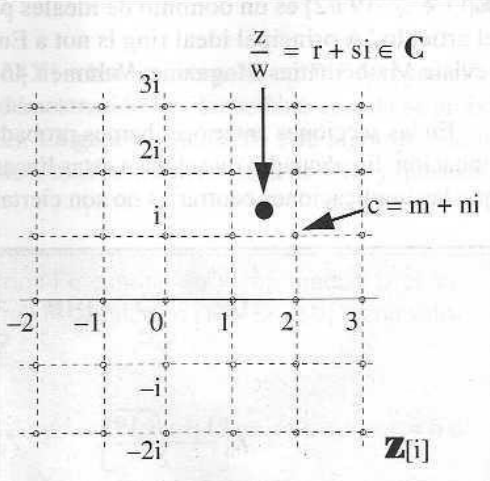
\includegraphics[scale=0.5]{./images/approximation.png}
	}
\end{figure}

\begin{example}[Resolución de ecuaciones lineales en los enteros de Gauss]
	Resolver la ecuación $2ix = 11i$ en $\mathbb{Z}[i]$ equivale a comprobar si $2i$ divide a $11i$. lo que en un dominio euclídeo implica ver que todo resto euclídeo es cero. Consideramos la fracción $\frac{11+7i}{2i}$ y la racionalizamos multiplicando denominador y numerador mediante $-2i$ obteniendo $\frac{-22i+14}{4} = \frac{-11i+7}{2}$ y por tanto $q = -6i+4$ y $r = (-6i+4)(11+7i) = -i+1$. El resto obtenido aquí es un resto euclídeo que no es cero. Por tanto, la ecuación no tiene solución. 
	
	En cambio, la ecuación $(7+2\sqrt{2})x = 4 + 7 \sqrt{2}$ tiene como única solución $x = \sqrt{2}$.
\end{example}

